\documentclass[a4paper]{article}

\usepackage[english]{babel}
\usepackage[utf8]{inputenc}
\usepackage{amsmath}
\usepackage{graphicx}
\usepackage[colorinlistoftodos]{todonotes}

\usepackage{theorem}
\usepackage{amssymb}

\usepackage{hyperref}

\usepackage{caption}
\usepackage{subcaption}

\newenvironment{proof}{{\bf Proof:  }}{\hfill\rule{2mm}{2mm}}

\newtheorem{fact}{Fact}[section]
\newtheorem{lemma}[fact]{Lemma}
\newtheorem{theorem}[fact]{Theorem}
\newtheorem{definition}[fact]{Definition}
\newtheorem{corollary}[fact]{Corollary}
\newtheorem{proposition}[fact]{Proposition}
\newtheorem{claim}[fact]{Claim}
\newtheorem{exercise}[fact]{Exercise}

\newcommand{\RT}[1]{\marginpar{\footnotesize\color{red}RT: #1}}


\usepackage{tikz}
\usetikzlibrary{arrows}
\usepackage{amsmath}

\usepackage{algorithm}
\usepackage{algorithmic}
\usepackage{bm}

\renewcommand{\algorithmicrequire}{\textbf{Input:}}
\renewcommand{\algorithmicensure}{\textbf{Output:}}
\renewcommand{\hat}{\widehat}

% Defines a `datastore' shape for use in DFDs.  This inherits from a
% rectangle and only draws two horizontal lines.
\makeatletter
\pgfdeclareshape{datastore}{
  \inheritsavedanchors[from=rectangle]
  \inheritanchorborder[from=rectangle]
  \inheritanchor[from=rectangle]{center}
  \inheritanchor[from=rectangle]{base}
  \inheritanchor[from=rectangle]{north}
  \inheritanchor[from=rectangle]{north east}
  \inheritanchor[from=rectangle]{east}
  \inheritanchor[from=rectangle]{south east}
  \inheritanchor[from=rectangle]{south}
  \inheritanchor[from=rectangle]{south west}
  \inheritanchor[from=rectangle]{west}
  \inheritanchor[from=rectangle]{north west}
  \backgroundpath{
    %  store lower right in xa/ya and upper right in xb/yb
    \southwest \pgf@xa=\pgf@x \pgf@ya=\pgf@y
    \northeast \pgf@xb=\pgf@x \pgf@yb=\pgf@y
    \pgfpathmoveto{\pgfpoint{\pgf@xa}{\pgf@ya}}
    \pgfpathlineto{\pgfpoint{\pgf@xb}{\pgf@ya}}
    \pgfpathmoveto{\pgfpoint{\pgf@xa}{\pgf@yb}}
    \pgfpathlineto{\pgfpoint{\pgf@xb}{\pgf@yb}}
 }
}
\makeatother



\title{Outline for Robust LLG}

\date{\today}

\begin{document}
\maketitle

\section{Background and Overview}

\begin{itemize}

\item Network analysis is becoming more and more widely used recently. In a general parametric framework, $G \sim F \in \mathcal{F} = \{F_{\theta} : \theta \in \Theta \}$, selecting a reasonable estimator $\hat{\theta}(G)$ for the unknown $\theta$ given a finite graph sample $G$ is one of the most important tasks.

\item In the most basic setting, i.e. undirected graphs with each edge distributed Bernoulli independently, the parameters are the probabilities of the existence of edges between all pair of vertices.
Then the element-wise maximum likelihood estimate, which happens to be the sample mean in this situation, is the uniformly minimum-variance unbiased estimator if we only consider the independent edge graph model \cite{bollobas2007phase} without taking any graph structure into account. However, it does not perform very well especially when we only have a few observations, which is likely the case in real world.

\item One of the most important structures about the networks is the community structure in which vertices are clustered into different communities such that vertices of the same community behave similarly. The stochastic blockmodel (SBM) \cite{holland1983stochastic} captures such structural property and is widely used in modeling networks.
Meanwhile, the latent positions model (LPM) \cite{hoff2002latent}, a much more general model compared to SBM, proposes a way to parameterize the graph structure by latent positions associated with each vertex. However, the random dot product graph (RDPG) \cite{young2007random, nickel2007random} which is a special case of LPM stays in between and motivates our estimator.

\item The Law of Large Graphs \cite{tang2016law} considers a low-rank approximation of the sample mean graph as an estimator motivated by the RDPG model and proves that in the basic Bernoulli setting under SBM, the new estimator outperforms the element-wise MLE since it decreases the overall variance dramatically compare to the naive entry-wise sample mean by biasing towards the low-rank structure. 

\item While the Law of Large Graphs considers an estimator which captures the low-rank structure and demonstrates its improvement over the entry-wise MLE for the unweighted graphs with Bernoulli distribution, a more generalized setting is always preferred.

\item Firstly, we extend the unweighted graphs with Bernoulli distribution to weighted graphs with a general distribution $F$. Then all the models we mentioned above could be modified naturally and are discussed in details in Section \ref{section:WIEM}, \ref{section:WRDPG} and \ref{section:WSBM}.

\item Also in the Law of Large Graphs paper, it is assumed that the adjacency matrix is observed without contamination, however in practice there will be noise in the observed graph. In this case, a contamination model, e.g. gross error model considered in this work \cite{AIC:AIC690280519, bickel2001mathematical}, is always preferred. In a gross error model, we observe good measurement $G^* \sim F_P \in \mathcal{F}$ most of the time, while there are a few wild values $G^{**} \sim H_C \in \mathcal{H}$ when the gross errors occur.
As to the graphs, one way to generalize from the gross error model is to contaminate the entire graph with some small probability $\epsilon$, that is $G \sim (1-\epsilon) F_P + \epsilon H_C$. However, since we are under the independent edge model, it is more natural to consider the contaminations on each edge, i.e. for $1 \le i < j \le n$, $G_{ij} \sim (1-\epsilon) F_{P_{ij}} + \epsilon H_{C_{ij}}$ with $F \in \mathcal{F}$ and $G \in \mathcal{G}$, where both $\mathcal{F}$ and $\mathcal{G}$ are one-parameter distribution families.

\item Under the contamination model, although we observe $G$ instead of $G^*$, estimating the parameters $P_{ij}$ ($1 \le i < j \le n$) of $F_{P_{ij}}$ in $\mathcal{F}$ is still our goal. We first proved that the estimator based on ASE ($\widetilde{P}^{(1)}$ in Figure \ref{fig:roadmap}) proposed in LLG is still better than entry-wise MLE ($\hat{P}^{(1)}$ in Figure \ref{fig:roadmap}) in MSE when the observations are contaminated under proper conditions.

\item Furthermore, with contaminations, it is more preferable to use robust methods, like ML$q$E \cite{ferrari2010, qin2013maximum} considered in this paper. We proved that entry-wise ML$q$E ($\hat{P}^{(q)}$ in Figure \ref{fig:roadmap}) improves the performance compared to entry-wise MLE ($\hat{P}^{(1)}$ in Figure \ref{fig:roadmap}) whenever contamination is relatively large.

\item Similarly, in order to take advantage of the low-rank structure, we enforce a low-rank approximation on the entry-wise ML$q$E. We prove that, under proper assumptions, the new estimator ($\widetilde{P}^{(q)}$ in Figure \ref{fig:roadmap}) not only inherits the robust property from ML$q$E ($\hat{P}^{(q)}$ in Figure \ref{fig:roadmap}), but also wins the bias-variance trade-off by taking advantage of the low-rank structure.

\end{itemize}



\begin{figure}
\begin{center}
\hspace*{-0.2in}
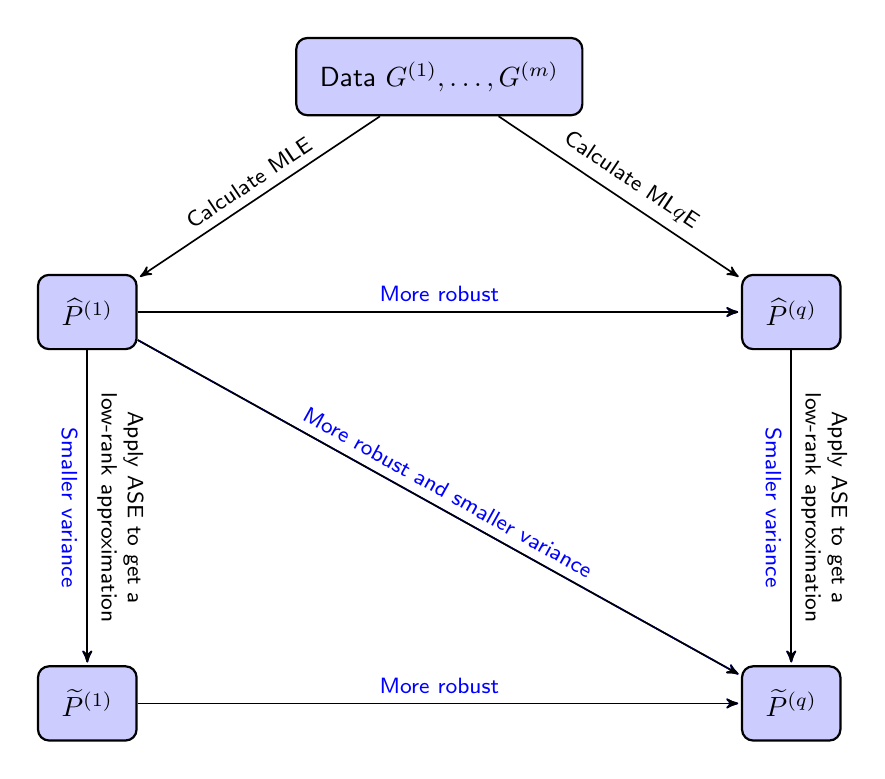
\begin{tikzpicture}[
  font=\sffamily,
  every matrix/.style={ampersand replacement=\&,column sep=2cm,row sep=2cm},
  block/.style={draw,thick,rounded corners,fill=blue!20,inner sep=.3cm},
  process/.style={draw,thick,circle,fill=blue!20},
  sink/.style={source,fill=green!20},
  datastore/.style={draw,very thick,shape=datastore,inner sep=.3cm},
  dots/.style={gray,scale=2},
  to/.style={->,>=stealth',shorten >=1pt,semithick,font=\sffamily\footnotesize},
  tofrom/.style={<->,>=stealth',shorten >=1pt,semithick,font=\sffamily\footnotesize},
  every node/.style={align=center}]

  % Position the nodes using a matrix layout
  \matrix{
  	\& \node[block] (Data) {Data $G^{(1)}, \dotsc, G^{(m)}$};\\
    \node[block] (MLE) {$\hat{P}^{(1)}$};
      \& \& \node[block] (MLqE) {$\hat{P}^{(q)}$};\\
	\\
    \node[block] (XMLE) {$\widetilde{P}^{(1)}$};
      \& \& \node[block] (XMLqE) {$\widetilde{P}^{(q)}$}; \\
  };

  % Draw the arrows between the nodes and label them.
  % \draw[to, blue] (Data) -- node[midway, sloped, below] {UMVUE w/o contamination} (MLE);
  \draw[to] (Data) -- node[midway, sloped, above] {Calculate MLE} (MLE);
  \draw[to] (Data) -- node[midway, sloped, above] {Calculate ML$q$E} (MLqE);
  \draw[to, blue] (MLE) -- node[midway,above] {More robust} (MLqE);
  \draw[to] (MLE) -- (MLqE);
  \draw[to, blue] (MLE) -- node[midway, sloped, below] {Smaller variance} (XMLE);
  \draw[to] (MLE) -- node[midway, sloped, above] {Apply ASE to get a \\ low-rank approximation} (XMLE);
  \draw[to, blue] (MLqE) -- node[midway, sloped, below] {Smaller variance} (XMLqE);
  \draw[to] (MLqE) -- node[midway, sloped, above] {Apply ASE to get a \\ low-rank approximation} (XMLqE);
  \draw[to, blue] (XMLE) -- node[midway,above] {More robust} (XMLqE);
  \draw[to] (XMLE) -- (XMLqE);
  \draw[to, blue] (MLE) -- node[midway, sloped, above] {More robust and smaller variance} (XMLqE);
  \draw[to] (MLE) -- (XMLqE);
\end{tikzpicture}
\end{center}
\caption{\label{fig:roadmap}Roadmap among the data and four estimators.}
\end{figure}


\section{Models}
\label{section:model}
\begin{itemize}
\item For this work, we are in the scenario where $m$ weighted graphs each with $n$ vertices are given in the adjacency matrices form $\{ A^{(t)} \} (t = 1, \dotsc, m)$. The graphs we consider in this work are undirected without self-loop, i.e. each $A^{(t)}$ is symmetric with zeros along the diagonal. Moreover, we assume the vertex correspondence is known throughout different graphs, so that vertex $i$ of graph $t_1$ corresponds to vertex $i$ of graph $t_2$ for any $i$, $t_1$, $t_2$.
\item In this section, we present three nested models, the weighted independent edge model in Section \ref{section:WIEM}, the weighted random dot product graph model in Section \ref{section:WRDPG}, and the weighted stochastic blockmodel (WSBM) as a WRDPG in Section \ref{section:WSBM}. Moreover, we introduce a contaminated model based on Section \ref{section:WSBM} in Section \ref{section:Contamination}.
\end{itemize}

\subsection{Weighted Independent Edge Model}
\label{section:WIEM}
\begin{itemize}
\item We first extend the definition of independent edge model (IEM) \cite{bollobas2007phase} to the weighted independent edge model (WIEM) corresponding to a one-parameter family $\mathcal{F} = \{ F_{\theta} : \theta \in \Theta \subset \mathbb{R} \}$. Denote the graph parameter as a matrix $P \in \Theta^{n \times n} \subset \mathbb{R}^{n \times n}$, then under a WIEM, each edge between vertex $i$ and vertex $j$ ($i < j$ because of symmetry) is distributed from $F_{P_{ij}}$ independently.
\item A simple example here is a WIEM for binary graphs with respect to $\mathcal{F}$ to be Bernoulli with a symmetric and hollow parameter matrix $P \in [0, 1]^{n \times n}$.
\item Note that the graphs considered in this paper are undirected without self-loop, thus the parameter matrix $P$ needs to be symmetric and hollow. However, for convenience, we still define the parameters to be an $n$-by-$n$ matrix while only $n \choose 2$ of them are effective.
\end{itemize}

\subsection{Weighted Random Dot Product Graph}
\label{section:WRDPG}
\begin{itemize}
\item The connectivity between two vertices in a graph generally depends on some hidden properties of the corresponding vertices. The latent positions model proposed by Hoff et al. \cite{hoff2002latent} captures such properties by assigning each vertex $i$ with a corresponding latent vector $X_i \in \mathbb{R}^d$. Conditioned on the latent vectors $X_i$ and $X_j$, the edge between vertex $i$ and vertex $j$ is independent of all other edges and depends only on $X_i$ and $X_j$ through a link function. This can easily be generalized to the weighted version easily.
\item A special case of the latent position model is the random dot product graph model (RDPG) in which the link function is the inner product \cite{young2007random, nickel2007random}. In the following, we give a definition of the weighted random dot product graph (WRDPG) as a generalization of the weighted latent positions model.
\begin{definition}
Consider a collection of one-parameter distributions $\mathcal{F} = \{ F_{\theta}, \theta \in \Theta \subset \mathbb{R} \}$. Then the weighted random dot product graph model (WRDPG) with respect to $\mathcal{F}$ is defined as following: Let $\boldsymbol{X} \in \mathbb{R}^{n \times d}$ be such that $\boldsymbol{X} = [X_1, X_2, \dotsc, X_n]^T$, where $X_i \in \mathbb{R}^d$ for all $i \in [n]$. The matrix $\boldsymbol{X}$ is random and satisfies $\mathbb{P}\left[ \langle X_i, X_j \rangle \in \Theta \right] = 1$ for all $i, j \in [n]$. Conditioned on $\boldsymbol{X}$, the entries of the adjacency matrix $\boldsymbol{A}$ are independent and $\boldsymbol{A}_{ij}$ is a random variable with distribution $F \in \mathcal{F}$ with parameter $\langle X_i, X_j \rangle$ for all $i \ne j \in [n]$.
\end{definition}
Under the WRDPG defined above, the parameter matrix $P = X X^T \in \mathbb{R}^{n \times n}$ is automatically symmetric because the link function is inner product. Moreover, to have symmetric graphs without self-loop, only $A_{ij}$ ($i < j$) are sampled while leaving the diagonals of $A$ to be all zeros.

%\begin{definition}
%Consider a collection of one-parameter distributions $\mathcal{F} = \{ F_{\theta}, \theta \in \Theta \subset \mathbb{R} \}$. Then the weighted random dot product graph model (WRDPG) with respect to $\mathcal{F}$ is defined as following: Let $\boldsymbol{X}, \boldsymbol{Y} \in \mathbb{R}^{n \times d}$ be such that $\boldsymbol{X} = [X_1, X_2, \cdots, X_n]^T$ and $\boldsymbol{Y} = [Y_1, Y_2, \cdots, Y_n]^T$, where $X_u, Y_u \in \mathbb{R}^d$ for all $u \in [n]$. The matrices $\boldsymbol{X}$ and $\boldsymbol{Y}$ are random and satisfy $\mathbb{P}\left[ \langle X_u, Y_v \rangle \in \Theta \right] = 1$ for all $u, v \in [n]$. Conditioned on $\boldsymbol{X}$ and $\boldsymbol{Y}$, the entries of the adjacency matrix $\boldsymbol{A}$ are independent and $\boldsymbol{A}_{uv}$ is a random variable with distribution $f \in \mathcal{F}$ with parameter $\langle X_u, Y_v \rangle$ for all $u \ne v \in [n]$.
%\end{definition}
\end{itemize}

\subsection{Weighted Stochastic Blockmodel as a Weighted Random Dot Product Graph}
\label{section:WSBM}
\begin{itemize}
\item Community structure is an important property of graphs under which vertices are clustered into different communities such that vertices within the same community behave similarly. The stochastic blockmodel (SBM) \cite{holland1983stochastic} captures such property, where each vertex is assigned to one block and the connectivity between two vertices depends only on their respective block memberships.
\item Formally, the SBM is determined by the number of blocks $K$ (generally much smaller than the number of vertices $n$), block probability matrix $B \in \Theta^{K \times K} \subset \mathbb{R}^{K \times K}$, and the block assignment vector $\tau \in [K]^n$, where $\tau_i = k$ represents vertex $i$ belongs to block $k$. Conditioned on the block membership $\tau$, the connectivity between vertex $i$ and vertex $j$ follows a Bernoulli distribution with parameter $B_{\tau_i, \tau_j}$. This can easily be generalized to the weighted stochastic blockmodel (WSBM), by substituting the Bernoulli distribution to a general distribution family $\mathcal{F}$.
\item In order to consider WSBM as a WRDPG, the matrix $B$ needs to be positive semi-definite. From now on, we will note the sub-model of WSBM with positive semi-definite $B$ as the WSBM.
\item Now consider the WSBM as a WRDPG with respect to $\mathcal{F} = \{ F_{\theta}, \theta \in \Theta \subset \mathbb{R} \}$. Let $d = 
\mathrm{rank}(B)$, then all vertices in block $k$ have shared latent position $\nu_k \in \mathbb{R}^{d}$, where $B = \nu \nu^{\top}$ and $\nu = [\nu_1, \dotsc, \nu_K]^{\top} \in \mathbb{R}^{K \times d}$. That is to say, $X_i = \nu_{\tau_i}$ and $A_{ij}$ $(i < j)$ is distributed from $F$ with parameter $B_{\tau_i, \tau_j} = \nu_{\tau_i}^{\top} \nu_{\tau_j}$. Here the parameter matrix $P \in \mathbb{R}^{n \times n}$ is symmetric, hollow, and satisfies $P_{ij} = X_i^{\top} X_j = \nu_{\tau_i}^{\top} \nu_{\tau_j} = B_{\tau_i, \tau_j}$.
\item In order to generate $m$ graphs under this model with known vertex correspondence, we first sample $\tau$ from the categorical distribution with parameter $\rho$ and keep it fixed for all $m$ graphs. Then $m$ symmetric and hollow graphs $G^{(1)}, \dotsc, G^{(m)}$ are sampled such that conditioning on $\tau$, the adjacency matrices are distributed entry-wise independently as $A^{(t)}_{ij} \stackrel{ind}{\sim} F_{B_{\tau_i, \tau_j}} = F_{P_{ij}}$ for each $1 \le t \le m$, $1 \le i < j \le n$. Here $P \in \mathbb{R}^{n \times n}$ is the actual parameter matrix for each pair of vertices with the same block structure as $B$.
\item Here is an example of the SBM. (Figure for simulation)
\end{itemize}

\subsection{Stochastic Blockmodel as a Weighted Random Dot Product Graph with Contaminations}
\label{section:Contamination}
\begin{itemize}
\item In practice, we always get noise in the observations, which deviates from our general model assumptions. In order to incorporate this effect, a contamination model, e.g. gross error model \cite{AIC:AIC690280519, bickel2001mathematical} considered in this work, is always preferred.
\item Generally in a gross error model, we observe good measurement $G^* \sim F_P \in \mathcal{F}$ most of the time, while there are a few wild values $G^{**} \sim H_C \in \mathcal{H}$ when the gross errors occur. Here $P$ and $C$ represent the respective parameter matrices for the two distribution families.
As to the graphs, one way is to contaminate the entire graph with some small probability $\epsilon$, that is $G \sim (1-\epsilon) F_P + \epsilon H_C$. However, since we are under the independent edge model, it is more natural to consider the contaminations on each edge, i.e. for $1 \le i <  j \le n$, $G_{ij} \sim (1-\epsilon) F_{P_{ij}} + \epsilon H_{C_{ij}}$ with $F \in \mathcal{F}$ and $G \in \mathcal{G}$, where both $\mathcal{F}$ and $\mathcal{G}$ are one-parameter distribution families.
\item In this paper, we assume that when gross errors occur, the connectivity also follows the WSBM as a WRDPG. That is, the contamination distributions $H_{C_{ij}}$ are also from the same one-parameter family $\mathcal{F}$ as $F_{P_{ij}}$ do. Moreover, the parameter matrix $C$ for the contamination has the same block structure. (Note: not necessarily the same block structure)
\item To generate $m$ graphs under this contamination model with known vertex correspondence, we first sample $\tau$ from the categorical distribution with parameter $\rho$ and keep it fixed for all $m$ graphs as in Section \ref{section:WSBM}. Then $m$ symmetric and hollow graphs $G^{(1)}, \dotsc, G^{(m)}$ are sampled such that conditioning on $\tau$, the adjacency matrices are distributed entry-wise independently as $A^{(t)}_{ij} \stackrel{ind}{\sim} (1-\epsilon) F_{P_{ij}} + \epsilon F_{C_{ij}}$ for each $1 \le t \le m$, $1 \le i < j \le n$. Here $\epsilon$ is the probability of an edge to be contaminated, $P$ is the parameter matrix as in Section \ref{section:WSBM}, and $C$ is the parameter matrix for contaminations.
\end{itemize}



\section{Estimators}

Under each of the models mentioned in Section \ref{section:model}, our goal is to estimate the parameter matrix $P$ based on the $m$ observations $A^{(1)}, \dotsc, A^{(m)}$. In this section, we present four estimators as in Figure \ref{fig:roadmap}, the standard entry-wise MLE $\hat{P}^{(1)}$, the low-rank approximation of the entry-wise MLE $\widetilde{P}^{(1)}$, the entry-wise robust estimator ML$q$E $\hat{P}^{(q)}$, and the low-rank approximation of the entry-wise ML$q$E $\widetilde{P}^{(q)}$. Since the observed graphs are symmetric and hollow with a symmetric parameter matrix of the model, we don't really care about the estimate of the diagonal of $P$, but the estimate itself should be at least symmetric.

\subsection{Entry-wise Maximum Likelihood Estimator $\hat{P}^{(1)}$}
\begin{itemize}
\item Under the WIEM, the most natural estimator is the element-wise MLE $\hat{P}^{(1)}$ based on the adjacency matrices $A^{(1)}, \dotsc, A^{(m)}$.
\item In some cases, for instance Bernoulli, Exponential, and Poisson, the entry-wise MLE happens to be the mean graph $\bar{A}$, which is the UMVUE under WIEG with no other constraints. So it has the smallest variance among all unbiased estimators. In addition, as being an MLE, it satisfies many good asymptotic properties as the number of graphs $m \to \infty$. But the performance will not get any better when the number of vertices in each graph $n$ increases. In addition, it doesn't exploit any graph structure. If the graphs are actually distributed under a WRDPG or a WSBM, then the entry-wise MLE is no longer the MLE any more. As a result, the performance can be very poor, especially when $m$ is small.
\end{itemize}



\subsection{Estimator $\widetilde{P}^{(1)}$ Based on Adjacency Spectral Embedding of $\hat{P}^{(1)}$}
\begin{itemize}
\item Motivated by the low-rank structure of the parameter matrix $P$ in WRDPG, we consider the estimator $\widetilde{P}^{(1)}$ proposed by Tang et al. \cite{tang2016law} based on the spectral decomposition of $\hat{P}^{(1)}$. The estimator $\widetilde{P}^{(1)}$ is similar to the estimator proposed by Chaterjee \cite{chatterjee2015matrix} with adjustment for the specific estimation task, including a different dimension selection technique and a diagonal augmentation procedure.
\end{itemize}

\subsubsection{Rank-$d$ Approximation}
\begin{itemize}
\item Given the dimension $d$, we consider the best rank-$d$ positive semi-definite approximation of $\hat{P}^{(1)}$, denoted as $\widetilde{P}^{(1)}$. First calculate the eigen-decomposition of the symmetric matrix $\hat{P}^{(1)} = \hat{U} \hat{S} \hat{U}^{\top} + \widetilde{U} \widetilde{S} \widetilde{U}^{\top}$, where $\hat{S}$ is the diagonal matrix with the largest $d$ eigenvalues of $\hat{P}^{(1)}$, and $\hat{U}$ has the corresponding eigenvectors as each column. Then the best rank-$d$ positive semi-definite approximation is $\widetilde{P}^{(1)} = \hat{U} \hat{S} \hat{U}^{\top}$. Note that the $d$-dimensional adjacency spectral embedding (ASE) here is defined as $\hat{X} = \hat{U} \hat{S}^{1/2} \in \mathbb{R}^{n \times d}$. Thus the low rank approximation of $\hat{P}^{(1)}$ can also be represented as $\hat{X} \hat{X}^{\top}$. In the RDPG setting, Sussman et al. \cite{sussman2014consistent} proved that each row of $\hat{X}$ can accurately estimate the the latent position for each vertex up to an orthogonal transformation. We will analyze its performance under the WRDPG setting in Section \ref{section:theory}.
\item We restate the algorithm in \cite{tang2016law} to give the steps of computing this low-rank approximation of a general $n$-by-$n$ symmetric matrix $A$ in Algorithm \ref{algo:lowrank}.
\end{itemize}
\begin{algorithm}[H]
\caption{Algorithm to compute the rank-$d$ approximation of a matrix.}
\label{algo:lowrank}
\begin{algorithmic}[1]
\REQUIRE Symmetric matrix $A\in \mathbb{R}^{n \times n}$ and dimension $d\leq n$.
\ENSURE $\mathrm{lowrank}_d(A)\in \mathbb{R}^{n \times n}$
\STATE Compute the algebraically largest $d$ eigenvalues of $A$, $s_1\geq s_2\ge \dotsc \ge s_d$ and corresponding unit-norm eigenvectors $u_1,u_2,\dotsc,u_d\in \mathbb{R}^n$;
\STATE Set $\hat{S}$ to the $d\times d$ diagonal matrix $\mathrm{diag}(s_1,\dotsc,s_d)$;
\STATE Set $\hat{U} = [u_1,\dotsc,u_d]\in \mathbb{R}^{n \times d}$;
\STATE Set $\mathrm{lowrank}_d(A)$ to $\hat{U}\hat{S}\hat{U}^T$;
\end{algorithmic}
\end{algorithm}

\subsubsection{Dimension Selection}
\label{section:dim_select}
\begin{itemize}
\item A general way to choose the dimension $d$ in a dimension reduction setting is based on analyzing the ordered eigenvalues and looking for the ``gap'' or ``elbow'' in the scree-plot.
\item In 2006, Zhu and Ghodsi proposed an automatic method for finding the gap in the scree-plot by only looking at the eigenvalues based on a Gaussian mixture model \cite{zhu2006automatic}. Generally, the method provides multiple results based on different ``elbow''. In this paper, to avoid under-estimating the dimension, which is often much more harmful than over-estimating it, we always choose the 3rd elbow.
\item Although it is always challenge to choose a proper dimension, based on the (try simulation?) and real data experiment, a wide range of dimensions will lead to results nearly optimal. Thus a proper dimension selection method can be applied directly without carefully tuning the parameter, which is much more practical.
\end{itemize}

\subsubsection{Diagonal Augmentation}
\label{section:diag_aug}
\begin{itemize}
\item Since the graphs considered in this paper have no self-loops, all the adjacency matrices $A^{(t)}$ ($1 \le t \le m$) are hollow, i.e. all diagonal entries are zeros. And thus the diagonal of the parameter matrix $P$ doesn't matter since all off-diagonal entries are independent of them conditioned on the off-diagonal entries of $P$.
\item However, unlike the entry-wise estimators, e.g. $\hat{P}^{(1)}$, the ones which take advantage of the graph structure need the information from the diagonals. As a result, the zero diagonals of the observed graphs will lead to biased estimates. 
\item To compensate for such inaccurate estimate, Marchette et al. \cite{marchette2011vertex} suggested to use the average of the non-diagonal entries of the corresponding row as the diagonal entry before embedding. Also, Scheinerman and Tucker \cite{scheinerman2010modeling} proposed an iterative method, which gives a different approach to resolve such issue.
\item As suggested in \cite{tang2016law}, in this work we are going to combine both ideas by first using Marchette's row-averaging method (see Step 3 of Algorithm \ref{algo:basic}) and then another one-step Scheinerman's iterative method (see Step 6 of Algorithm \ref{algo:basic}).
\end{itemize}

\begin{algorithm}[H]
\caption{Algorithm to compute $\widetilde{P}^{(1)}$}
\label{algo:basic}
\begin{algorithmic}[1]
\REQUIRE Adjacency matrices $A^{(1)}, A^{(2)}, \dotsc, A^{(m)}$, with each $A^{(t)} \in \{0,1\}^{n \times n}$
\ENSURE Estimate $\widetilde{P}^{(1)} \in \mathbb{R}^{n \times n}$
\STATE Calculate the entry-wise MLE $\hat{P}^{(1)}$;
\STATE Calculate the scaled degree matrix $D = \mathrm{diag}(\hat{P}^{(1)} \bm{1})/(n-1)$;
\STATE Select the dimension $d$ based on the eigenvalues of $\hat{P}^{(1)} + D$; (see Section~\ref{section:dim_select})
\STATE Set $Q$ to $\mathrm{lowrank}_d(\hat{P}^{(1)} + D)$; (see Algorithm~\ref{algo:lowrank})
\STATE Set $D^{\prime}$ to $ \mathrm{diag}(Q)$, the diagonal matrix with diagonal matching $Q$; 
\STATE Set $Q^{\prime}$ to $\mathrm{lowrank}_d(Q + D^{\prime})$; (see Algorithm~\ref{algo:lowrank})
\STATE Set $\widetilde{P}^{(1)}$ to $Q^{\prime}$ with values $<0$ set to $0$.
\end{algorithmic}
\end{algorithm}

\begin{itemize}
\item Detailed description of the estimator $\widetilde{P}^{(1)}$ are given in Algorithm \ref{algo:basic}.
\end{itemize}

\subsection{Entry-wise Maximum L$q$ Likelihood Estimator $\hat{P}^{(q)}$}
\begin{itemize}
\item Motivated by the contamination
\item The MLE is asymptotically efficient, i.e. when sample size is large enough, the MLE is at least as accurate as any other estimator. However, when the sample size is moderate, robust estimators always outperforms MLE in terms of mean squared error by winning the bias-variance tradeoff.
\item Moreover, in practice, the observations are generally contaminated. In this case, robust estimators can even beat MLE asymptotically.
\item The class of parametric estimators based on the $q$-entropy function, the ML$q$E, is considered in this paper.
\end{itemize}


\subsection{Estimator $\widetilde{P}^{(q)}$ Based on Adjacency Spectral Embedding $\hat{P}^{(q)}$}
\begin{itemize}
\item Intuitively, the low rank structure of the WRDPG should be preserved more or less in the entry-wise ML$q$E.
\item Similarly, in order to take advantage of such low rank structure, we apply the same idea for building $\widetilde{P}^{(1)}$, i.e. enforce a low rank approximation on the entry-wise ML$q$E matrix $\hat{P}^{(q)}$ to get $\widetilde{P}^{(q)}$.
\item Detailed description of the algorithm for our estimator $\widetilde{P}^{(q)}$.
\end{itemize}


%\begin{figure}
%\centering
%\begin{subfigure}{.5\textwidth}
%  \centering
%  \includegraphics[width=1.2\linewidth]{SBM_P.png}
%\end{subfigure}%
%\begin{subfigure}{.5\textwidth}
%  \centering
%  \includegraphics[width=1.2\linewidth]{SBM_A.png}
%\end{subfigure}
%\caption{Example illustrating the SBM. The figure on the left is the probability matrix $P$ that follows a SBM with $K = 5$ blocks; The other figure shows the adjacency matrix $A$ for 200 vertices generated from the SBM with probability matrix $P$.}
%\label{fig:SBM_example}
%\end{figure}



\section{Theoretical Results}
\label{section:theory}
In this section, for illustrative purpose, we are going to present theoretical results when the contaminated model is based on exponential distributions, i.e. $\mathcal{F} = \{ f_{\theta}(x) = \frac{1}{\theta} e^{-x/\theta}, \theta \in [0, R] \subset \mathbb{R} \}$, where $R > 0$ is a constant. The results can be extended to a general situation with proper assumptions, which will be discussed in Section \ref{section:extension}.

\subsection{$\hat{P}^{(q)}$ vs $\hat{P}^{(1)}$}
\begin{lemma}
\label{lemma:ELqlEMLE}
For any $0 < q < 1$, there exists $C_0(P_{ij}, \epsilon, q) > 0$ such that under the contaminated model with $C > C_0(P_{ij}, \epsilon, q)$,
\[
	\lim_{m \to \infty} \left| E[\hat{P}^{(q)}_{ij}] - P_{ij} \right| < 
    \lim_{m \to \infty} \left| E[\hat{P}^{(1)}_{ij}] - P_{ij} \right|,
\]
for $1 \le i, j, \le n$ and $i \ne j$.
\end{lemma}

\begin{lemma}
\[
	\lim_{m \to \infty} \mathrm{Var}(\hat{P}^{(1)}_{ij})
    = \lim_{m \to \infty} \mathrm{Var}(\hat{P}^{(q)}_{ij}) = 0,
\]
for $1 \le i, j \le n$.
\end{lemma}


\subsection{$\widetilde{P}^{(1)}$ vs $\hat{P}^{(1)}$}
\begin{corollary}
\label{cor:L1Consistent}
Assuming that $m = O(n^b)$ for any $b > 0$, then the estimator based on ASE of MLE has the same entry-wise asymptotic bias as MLE, i.e.
\[
	\lim_{n \to \infty} \mathrm{Bias}(\widetilde{P}_{ij}^{(1)}) = \lim_{n \to \infty} E[\widetilde{P}_{ij}^{(1)}] - P_{ij} = \lim_{n \to \infty} E[\hat{P}^{(1)}_{ij}] - P_{ij}
    = \lim_{n \to \infty} \mathrm{Bias}(\hat{P}_{ij}^{(1)}).
\]
\end{corollary}

\begin{theorem}
\label{thm:VarASEL1}
Assuming that $m = O(n^b)$ for any $b > 0$, then $\mathrm{Var}((\hat{Z}_i^T \hat{Z}_j)_{\mathrm{tr}}) = O(m^{-1} n^{-2} (\log n)^6)$.
\end{theorem}

\begin{theorem}
\label{thm:AREL1}
For fixed $m$, $1 \le i, j \le n$ and $i \ne j$,
\[
	\frac{\mathrm{Var}(\widetilde{P}_{ij}^{(1)})}{\mathrm{Var}(\hat{P}_{ij}^{(1)})}
    = O(n^{-2} (\log n)^6).
\]
Thus
\[
	\mathrm{ARE}(\hat{P}_{ij}^{(1)}, \widetilde{P}_{ij}^{(1)}) = 0.
\]
Furthermore, as long as $m$ goes to infinity of order $O(n^b)$ for any $b > 0$,
\[
	\mathrm{ARE}(\hat{P}_{ij}^{(1)}, \widetilde{P}_{ij}^{(1)}) = 0.
\]
\end{theorem}





\subsection{$\widetilde{P}^{(q)}$ vs $\hat{P}^{(q)}$}
\begin{corollary}
\label{cor:LqConsistent}
Assuming that $m = O(n^b)$ for any $b > 0$, then the estimator based on ASE of ML$q$E has the same entry-wise asymptotic bias as ML$q$E, i.e.
\[
	\lim_{n \to \infty} \mathrm{Bias}(\widetilde{P}_{ij}^{(q)}) = \lim_{n \to \infty} E[\widetilde{P}_{ij}^{(q)}] - P_{ij} = \lim_{n \to \infty} E[\hat{P}^{(q)}_{ij}] - P_{ij}
    = \lim_{n \to \infty} \mathrm{Bias}(\hat{P}_{ij}^{(q)}).
\]
\end{corollary}

\begin{theorem}
\label{thm:VarASELq}
Assuming that $m = O(n^b)$ for any $b > 0$, then $\mathrm{Var}((\hat{Z}_i^T \hat{Z}_j)_{\mathrm{tr}}) = O(n^{-2} (\log n)^6)$.
\end{theorem}

\begin{theorem}
\label{thm:ARELq}
For fixed $m$, $1 \le i, j \le n$,
\[
	\frac{\mathrm{Var}(\widetilde{P}_{ij}^{(q)})}{\mathrm{Var}(\hat{P}_{ij}^{(q)})}
    = O(m n^{-2} (\log n)^6).
\]
Thus
\[
	\mathrm{ARE}(\hat{P}_{ij}^{(q)}, \widetilde{P}_{ij}^{(q)}) = 0.
\]
Furthermore, as long as $m$ goes to infinity of order $o(n^2 (\log n)^{-6})$,
\[
	\mathrm{ARE}(\hat{P}_{ij}^{(q)}, \widetilde{P}_{ij}^{(q)}) = 0.
\]
\end{theorem}




\subsection{$\widetilde{P}^{(q)}$ vs $\widetilde{P}^{(1)}$}

\begin{theorem}
\label{thm:biasL1andLq}
For sufficiently large $n$ and $C$, any $1 \le i,j \le n$,
\[
	\lim_{m \to \infty} \mathrm{Bias}(\widetilde{P}_{ij}^{(1)})
    > \lim_{m \to \infty} \mathrm{Bias}(\widetilde{P}_{ij}^{(q)})
\]
\end{theorem}

\begin{theorem}
\label{thm:varianceL1andLq}
For any fixed $m$, any $1 \le i,j \le n$,
\[
	\lim_{n \to \infty} \mathrm{Var}(\widetilde{P}_{ij}^{(1)})
    = \lim_{n \to \infty} \mathrm{Var}(\widetilde{P}_{ij}^{(q)}) = 0.
\]
Furthermore, as long as $m$ goes to infinity of order $o(n^2 (\log n)^{-6})$, any $1 \le i,j \le n$,
\[
	\lim_{n \to \infty} \mathrm{Var}(\widetilde{P}_{ij}^{(1)})
    = \lim_{n \to \infty} \mathrm{Var}(\widetilde{P}_{ij}^{(q)}) = 0
\]
\end{theorem}






\subsection{Summary}
In summary, we plot the relationship among four estimators in Figure \ref{fig:summary}.

\begin{figure}
\begin{center}
\hspace*{-0.2in}
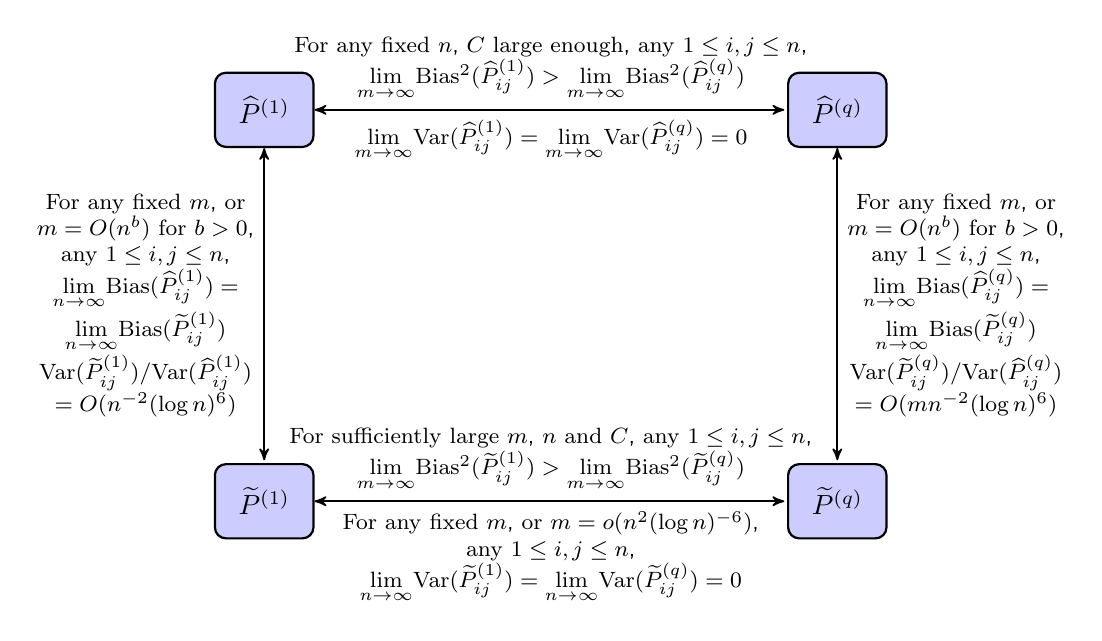
\begin{tikzpicture}[
  font=\sffamily,
  every matrix/.style={ampersand replacement=\&,column sep=2cm,row sep=2cm},
  block/.style={draw,thick,rounded corners,fill=blue!20,inner sep=.3cm},
  process/.style={draw,thick,circle,fill=blue!20},
  sink/.style={source,fill=green!20},
  datastore/.style={draw,very thick,shape=datastore,inner sep=.3cm},
  dots/.style={gray,scale=2},
  to/.style={->,>=stealth',shorten >=1pt,semithick,font=\sffamily\footnotesize},
  tofrom/.style={<->,>=stealth',shorten >=1pt,semithick,font=\sffamily\footnotesize},
  every node/.style={align=center}]

  % Position the nodes using a matrix layout
  \matrix{
    \node[block] (MLE) {$\hat{P}^{(1)}$};
      \& \& \& \node[block] (MLqE) {$\hat{P}^{(q)}$};\\
	\\
    \node[block] (XMLE) {$\widetilde{P}^{(1)}$};
      \& \& \& \node[block] (XMLqE) {$\widetilde{P}^{(q)}$}; \\
  };

  % Draw the arrows between the nodes and label them.
  \draw[tofrom] (MLE) -- node[midway,above] {$\mathrm{For}$ $\mathrm{any}$ $\mathrm{fixed}$ $n$, $C$ $\mathrm{large}$ $\mathrm{enough}$, $\mathrm{any}$ $1 \le i, j \le n$, \\$\underset{m \to \infty}{\lim} \mathrm{Bias}^2(\hat{P}_{ij}^{(1)}) > \underset{m \to \infty}{\lim} \mathrm{Bias}^2(\hat{P}_{ij}^{(q)})$}
      node[midway,below] {$\underset{m \to \infty}{\lim} \mathrm{Var}(\hat{P}_{ij}^{(1)}) = \underset{m \to \infty}{\lim} \mathrm{Var}(\hat{P}_{ij}^{(q)}) = 0$} (MLqE);
  \draw[tofrom] (MLE) -- node[midway,left] {$\mathrm{For}$ $\mathrm{any}$ $\mathrm{fixed}$ $m$, $\mathrm{or}$ \\ $m = O(n^b)$ $\mathrm{for}$ $b>0$, \\$\mathrm{any}$ $1 \le i, j \le n$, \\$\underset{n \to \infty}{\lim} \mathrm{Bias}(\hat{P}_{ij}^{(1)}) =$\\$ \underset{n \to \infty}{\lim} \mathrm{Bias}(\widetilde{P}_{ij}^{(1)})$\\$\mathrm{Var}(\widetilde{P}_{ij}^{(1)})/\mathrm{Var}(\hat{P}_{ij}^{(1)})$\\$ = O(n^{-2} (\log n)^6)$} (XMLE);
  \draw[tofrom] (MLqE) -- node[midway,right] {$\mathrm{For}$ $\mathrm{any}$ $\mathrm{fixed}$ $m$, $\mathrm{or}$ \\ $m = O(n^b)$ $\mathrm{for}$ $b>0$, \\$\mathrm{any}$ $1 \le i, j \le n$, \\$\underset{n \to \infty}{\lim} \mathrm{Bias}(\hat{P}_{ij}^{(q)}) = $\\$\underset{n \to \infty}{\lim} \mathrm{Bias}(\widetilde{P}_{ij}^{(q)})$\\$\mathrm{Var}(\widetilde{P}_{ij}^{(q)})/\mathrm{Var}(\hat{P}_{ij}^{(q)})$\\$= O(m n^{-2} (\log n)^6)$} (XMLqE);
  \draw[tofrom] (XMLE) -- node[midway,above] {$\mathrm{For}$ $\mathrm{sufficiently}$ $\mathrm{ large}$ $m$, $n$ $\mathrm{and}$ $C$, $\mathrm{any}$ $1 \le i, j \le n$, \\$\underset{m \to \infty}{\lim} \mathrm{Bias}^2(\widetilde{P}_{ij}^{(1)}) > \underset{m \to \infty}{\lim} \mathrm{Bias}^2(\widetilde{P}_{ij}^{(q)})$}
      node[midway,below] {$\mathrm{For}$ $\mathrm{any}$ $\mathrm{fixed}$ $m$, $\mathrm{or}$ $m = o(n^2 (\log n)^{-6})$, \\$\mathrm{any}$ $1 \le i, j \le n$, \\$\underset{n \to \infty}{\lim} \mathrm{Var}(\widetilde{P}_{ij}^{(1)}) = \underset{n \to \infty}{\lim} \mathrm{Var}(\widetilde{P}_{ij}^{(q)}) = 0$} (XMLqE);
\end{tikzpicture}
\end{center}
\caption{\label{fig:summary}Relationship among four estimators.}
\end{figure}






\section{Extensions}
\label{section:extension}
We can generalize both the exponential distribution and the entry-wise ML$q$E to an arbitrary $F$ and any entry-wise estimator $\hat{P}$ with the following assumptions:
\begin{itemize}
\item Let $A \stackrel{iid}{\sim} (1-\epsilon) F(P) + \epsilon F(C) $ and $H_{ij}^{(1)} = E[\hat{P}_{ij}^{(1)}] = (1-\epsilon) E_F(P_{ij}) + \epsilon E_F(C_{ij})$, then $E[(A_{ij} - H_{ij}^{(1)})^k] \le \mathrm{const} \cdot k!$.
\item There exists $C_0(P_{ij}, \epsilon) > 0$ such that under the contaminated model with $C > C_0(P_{ij}, \epsilon)$,
\[
	\lim_{m \to \infty} \left| E[\hat{P}_{ij}] - P_{ij} \right| < 
    \lim_{m \to \infty} \left| E[\hat{P}^{(1)}_{ij}] - P_{ij} \right|,
\]
for $1 \le i, j \le n$.
\item $\hat{P}_{ij} \le \mathrm{const} \cdot \hat{P}_{ij}^{(1)}$. This might be generalized to with high probability later.
\item $\mathrm{Var}(\hat{P}_{ij}) = O(m^{-1})$, where $m$ is the number of observations.
\end{itemize}

\section{Empirical Results}

\subsection{Simulation Results}

\begin{itemize}
\item We demonstrate the theoretical results in Section 3.1, the relative efficiency of $\hat{P}$, via various Monte Carlo simulation experiments.
\end{itemize}

\subsubsection{Simulation Setting}
\begin{itemize}
\item Here we consider the 2-block SBM parameterized by
\begin{equation*}
B = \begin{bmatrix}
4.2 & 2 \\
2 & 7
\end{bmatrix}
,\qquad \rho = \begin{bmatrix}
0.5 & 0.5
\end{bmatrix}.
\end{equation*}
\item The contamination is also a 2-block SBM parameterized by
\begin{equation*}
B = \begin{bmatrix}
20 & 18 \\
18 & 25
\end{bmatrix}
,\qquad \rho = \begin{bmatrix}
0.5 & 0.5
\end{bmatrix}.
\end{equation*}
\item And we embed the graphs into the dimension $d = \mathrm{rank}(B) = 2$.
\end{itemize}



\subsubsection{Simulation Results}
\begin{itemize}
\item Figure \ref{fig:eps} plots the mean squared error in average by varying contamination ratio $\epsilon$ with fixed $n = 100$ and $m = 10$ based on 1000 Monte Carlo replicates. And we use $q=0.8$ when applying ML$q$E.
Different colors represent the simulated MSE associated with four different estimators.
\textbf{1. MLE $\hat{P}^{(1)}$ vs ML$q$E $\hat{P}^{(q)}$:}
MLE outperforms a little bit when there is no contamination (i.e. $\epsilon = 0$), but it degrades dramatically when contamination increases;
\textbf{2. MLE $\hat{P}^{(1)}$ vs ASE o MLE $\widetilde{P}^{(1)}$: }
ASE procedure takes the low rank structure into account and $\widetilde{P}^{(1)}$ wins the bias-variance tradeoff;
\textbf{3. ML$q$E $\hat{P}^{(q)}$ vs ASE o ML$q$E $\widetilde{P}^{(q)}$: }
ML$q$E preserves the low rank structure of the original graph more or less, so ASE procedure still helps and $\widetilde{P}^{(q)}$ wins the bias-variance tradeoff;
\textbf{4. ASE o ML$q$E $\widetilde{P}^{(q)}$ vs ASE o MLE $\widetilde{P}^{(1)}$: }
When contamination is large enough, $\widetilde{P}^{(q)}$ based on ML$q$E is better, since it inherits the robustness from ML$q$E.
\item Figure \ref{fig:q} show the mean squared error in average by varying the parameter $q$ in ML$q$E with fixed $n = 100$, $m = 10$ and $\epsilon = 0.2$ based on 1000 Monte Carlo replicates. Different colors represent the simulated MSE associated with four different estimators.
1. ASE procedure takes advantage of the graph structure and improves the performance of the corresponding estimators;
2. ML$q$E shows the robustness property compare to the MLE. And as $q$ goes to 1, ML$q$E goes to the MLE as expected.
\item By comparing the performance of the four estimators based on different setting, we demonstrate the theoretical results in Section \ref{section:theory}.
\end{itemize}

\begin{figure}[!htb]
\centering
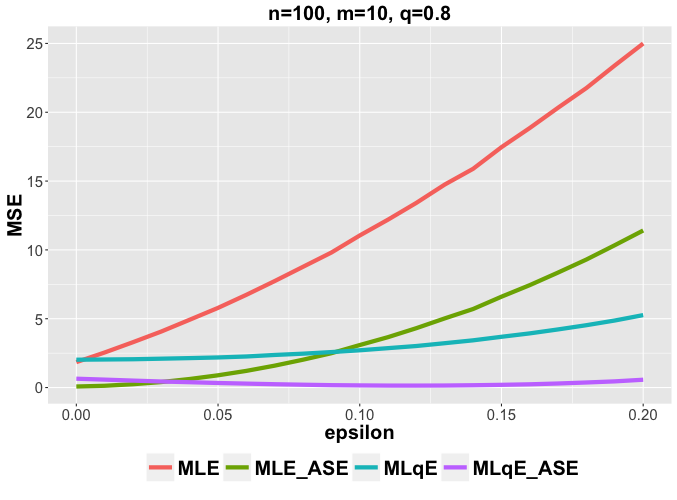
\includegraphics[width=1\textwidth]{eps.png}
\caption{Mean squared error in average by varying contamination ratio $\epsilon$ with fixed $n = 100$ and $m = 10$ based on 1000 Monte Carlo replicates. And we use $q=0.8$ when applying ML$q$E.
Different colors represent the simulated MSE associated with four different estimators.
\textbf{1. MLE $\hat{P}^{(1)}$ vs ML$q$E $\hat{P}^{(q)}$:}
MLE outperforms a little bit when there is no contamination (i.e. $\epsilon = 0$), but it degrades dramatically when contamination increases;
\textbf{2. MLE $\hat{P}^{(1)}$ vs ASE o MLE $\widetilde{P}^{(1)}$: }
ASE procedure takes the low rank structure into account and $\widetilde{P}^{(1)}$ wins the bias-variance tradeoff;
\textbf{3. ML$q$E $\hat{P}^{(q)}$ vs ASE o ML$q$E $\widetilde{P}^{(q)}$: }
ML$q$E preserves the low rank structure of the original graph more or less, so ASE procedure still helps and $\widetilde{P}^{(q)}$ wins the bias-variance tradeoff;
\textbf{4. ASE o ML$q$E $\widetilde{P}^{(q)}$ vs ASE o MLE $\widetilde{P}^{(1)}$: }
When contamination is large enough, $\widetilde{P}^{(q)}$ based on ML$q$E is better, since it inherits the robustness from ML$q$E.}
\label{fig:eps}
\end{figure}

\begin{figure}[!htb]
\centering
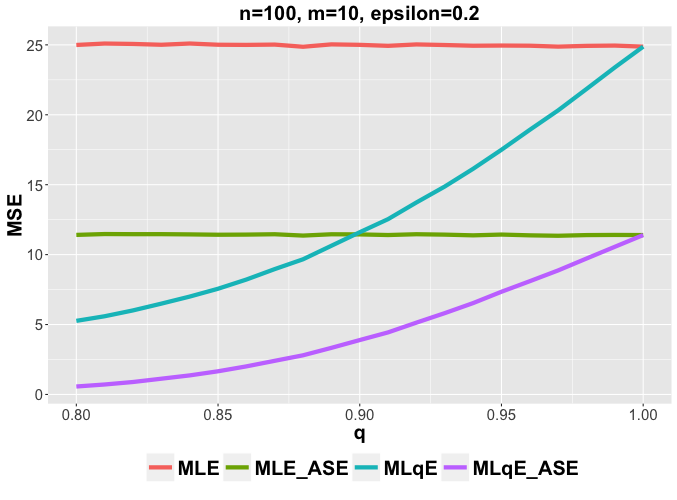
\includegraphics[width=1\textwidth]{q.png}
\caption{Mean squared error in average by varying the parameter $q$ in ML$q$E with fixed $n = 100$, $m = 10$ and $\epsilon = 0.2$ based on 1000 Monte Carlo replicates. Different colors represent the simulated MSE associated with four different estimators.
1. ASE procedure takes advantage of the graph structure and improves the performance of the corresponding estimators;
2. ML$q$E shows the robustness property compare to the MLE. And as $q$ goes to 1, ML$q$E goes to the MLE as expected.}
\label{fig:q}
\end{figure}

  
\begin{figure}
\centering
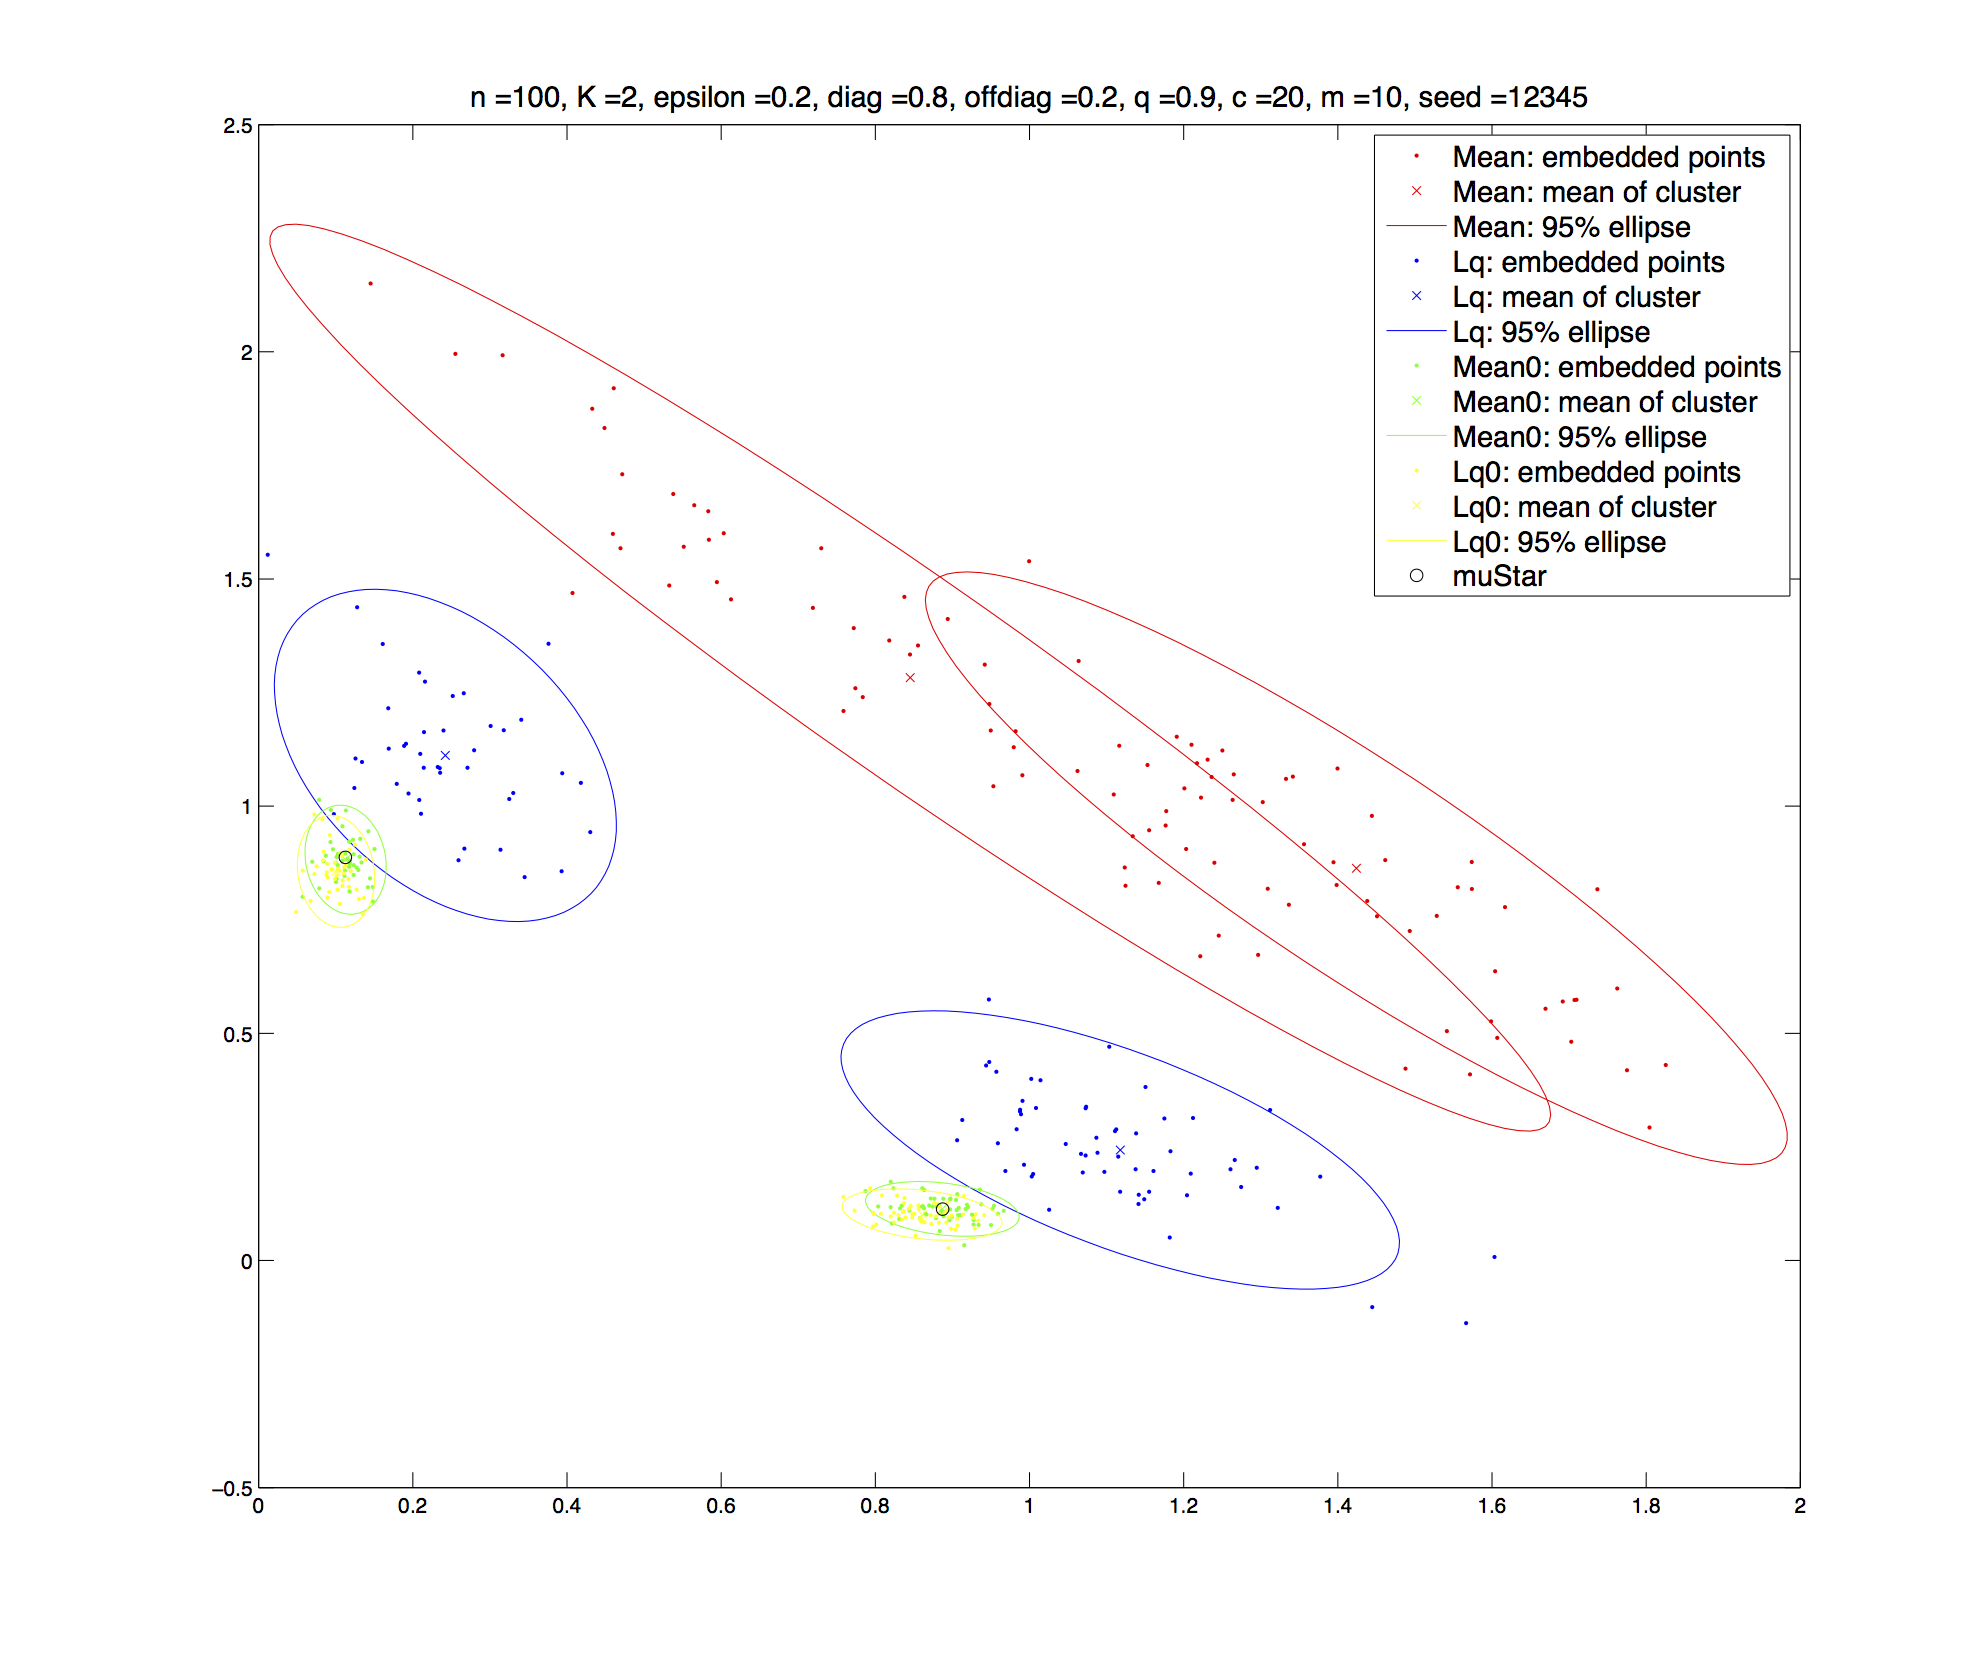
\includegraphics[width=0.8\textwidth]{Cluster.png}
\end{figure}



\subsection{CoRR Graphs}
\begin{itemize}
\item In practice, the graphs may not perfectly follow an RDPG, or even not IEM. But we are still interested in the discussed approach. To demonstrate that the estimates are still valid in such cases, we examine the datasets, CPAC200, which is a set of 454 brain connectomes with different number of nodes generated from fMRI scans available at the Consortium for Reliability and Reproducibility (CoRR).
\item The dataset has 454 different brain scans in the form of weighted, undirected graph with no self loop, based on the pipeline described in \cite{kiar2016graph} and \cite{neurodata}.
\item To compare the four estimators, we perform a cross-validation study on 454 graphs.
\item We run 1000 simulations on the dataset for each sample size $m = 1$, $m = 2$, $m = 5$. And we apply ASE for all possible dimensions, i.e. $d$ ranges from 1 to $n$. The result is shown in Figure \ref{fig:CPAC200}.
\item Since it is real data, ML$q$E outperforms ML$E$ because of the robustness property. Moreover, as suggested in the previous theorems, such property is kept after the ASE procedure.
\item When $d$ is small, ASE procedure underestimates the dimension and fail to get important information, which leads to poor performance. In practice, we use algorithms like Zhu and Ghodsi's method to select the dimension $d$. We can see Zhu and Ghodsi's algorithm does a pretty good job for selecting the dimension to embed.
\item When $m$ is small, MLE and ML$q$E have large variances which lead to large MSE. Meanwhile, the ASE procedure reduces the variance by taking advantages of the graph structure.
\end{itemize}

\begin{figure}
\centering
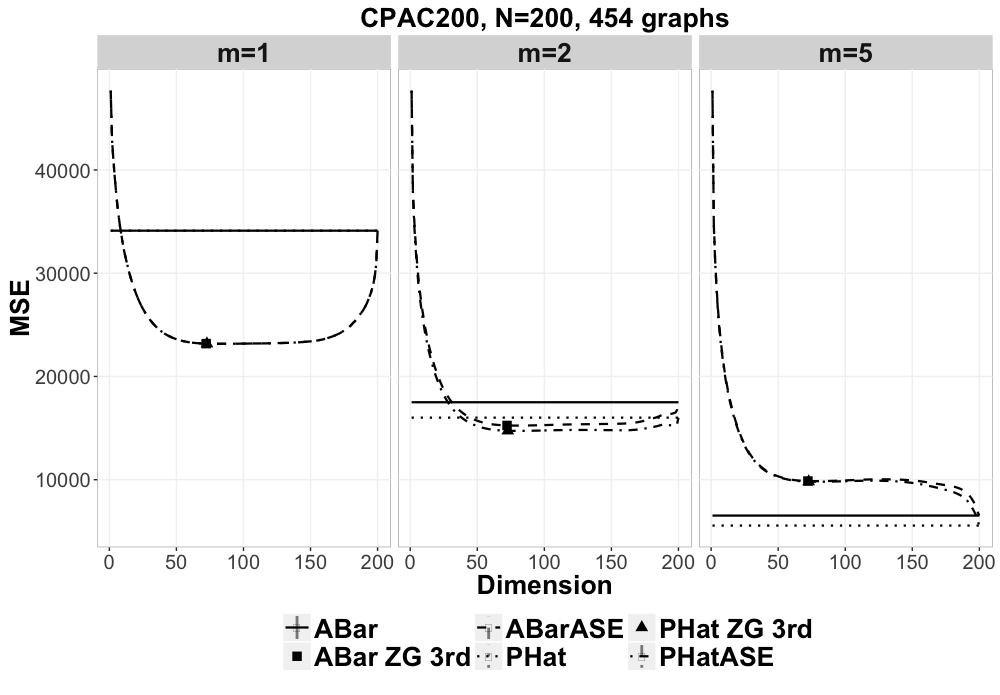
\includegraphics[width=0.8\textwidth]{CPAC200.png}
\caption{Comparison of mean squared error in average among four estimators while embedding the graphs into different dimensions with different size $m$ of the subsamples. The dimensions chosen by the 3d elbow of Zhu and Ghodsi are denoted in triangle and square. When $m$ is small, both robust estimation and ASE procedure help improving the performance, making $\widetilde{P}^{(q)}$ the best among four estimators.}
\label{fig:CPAC200}
\end{figure}





\section{Discussion}


\section{Appendix}

All proofs here.



\bibliography{Bib}{}
\bibliographystyle{plain}






%\newpage
%
%\section{Backup}
%
%
%\section{Discussion}
%
%\subsection{Summary}
%\begin{itemize}
%\item In this paper, we propose a better way to estimate the mean of a collection of graphs by taking advantage of the low rank structure of the graphs.
%\end{itemize}
%
%\subsection{Future Work}
%\begin{itemize}
%\item Generally the observations we have are always contaminated in practice. In this case, improved robust estimator based on the low rank structure of the graphs is preferred.
%\item Estimating the rank of the graph structure accurately will certainly help improve the results.
%\item In this paper, we are using Scheinerman's method with 1 iteration for diagonal augmentation.
%\end{itemize}
%
%
%
%
%
%
%\section{Methods}
%
%\subsection{Choosing Dimension}
%\label{section:dim_select}
%\begin{itemize}
%\item Often in dimensionality reduction techniques, the choice for dimension, d, relies on visually analyzing a plot of the ordered eigenvalues, looking for a ``gap'' or ``elbow'' in the scree-plot.
%\item USVT is a simple estimation procedure that works for any matrix that has ``a little bit of structure''.
%\end{itemize}
%
%\subsection{Graph Diagonal Augmentation}
%\begin{itemize}
%\item The graphs examined in this work are hollow, in that there are no self-loops and thus the diagonal entries of the adjacency matrix are 0. This leads to a bias in the calculation of the eigenvectors.
%\item We minimize this bias by using an iterative method developed by Scheinerman and Tucker.
%\end{itemize}
%
%\subsection{Source Code}
%
%\subsection{Dataset Description}
%\begin{itemize}
%\item The original dataset is from the Emotion and Creativity One Year Retest Dataset provided by Qiu, Zhang and Wei from Southwest University. It is comprised of 235 subjects, all of whom were college students. Each subject underwent two sessions of anatomical, resting state DTI scans, spaced one year apart. Due to the incomplete data, the true number of scans is 454.
%\item When deriving MR connectomes, the NeuroData team parcellate the brain into groups of nodes as defined by anatomical atlases. The atlases are defined either physiologically or structurally by neuroanatomists (Desikan and JHU), or are generated using a segmentation algorithm looking for certain features or groupings (CPAC200).
%\item The graphs we are using are processed by NeuroData team from DTI data of the original dataset generated with different atlases (desikan, JHU and CPAC200), each containing different region/node definitions.
%\item The graphs are undirected, unweighted and with no self-loops. An edge exists between two regions when there is at least one white-matter tract connecting the corresponding two parts of the brain.
%\end{itemize}
%
%\subsection{Outline for the Proof of the Theorems}



\end{document}